% THIS DOCUMENT IS FOLLOWS THE VOLERE TEMPLATE BY Suzanne Robertson
% and James Robertson
% ONLY THE SECTION HEADINGS ARE PROVIDED
%
% Initial draft from https://github.com/Dieblich/volere
%
% Risks are removed because they are covered by the Hazard Analysis
\documentclass[12pt]{article}

\usepackage{booktabs}
\usepackage{tabularx}
\usepackage{enumitem}
\usepackage{hyperref}
\usepackage{enumitem}
\usepackage{graphicx}
\usepackage{float}
\usepackage{placeins}
\usepackage{hanging}

\hypersetup{
  bookmarks=true,         % show bookmarks bar?
  colorlinks=true,      % false: boxed links; true: colored links
  linkcolor=red,          % color of internal links (change box color
  % with linkbordercolor)
  citecolor=green,        % color of links to bibliography
  filecolor=magenta,      % color of file links
  urlcolor=cyan           % color of external links
}

\newcommand{\lips}{\textit{Insert your content here.}}

%% Comments

\usepackage{color}

\newif\ifcomments\commentstrue %displays comments
%\newif\ifcomments\commentsfalse %so that comments do not display

\ifcomments
\newcommand{\authornote}[3]{\textcolor{#1}{[#3 ---#2]}}
\newcommand{\todo}[1]{\textcolor{red}{[TODO: #1]}}
\else
\newcommand{\authornote}[3]{}
\newcommand{\todo}[1]{}
\fi

\newcommand{\wss}[1]{\authornote{magenta}{SS}{#1}} 
\newcommand{\plt}[1]{\authornote{cyan}{TPLT}{#1}} %For explanation of the template
\newcommand{\an}[1]{\authornote{cyan}{Author}{#1}}

%% Common Parts

\newcommand{\progname}{ProgName} % PUT YOUR PROGRAM NAME HERE
\newcommand{\authname}{Team \#, Team Name
\\ Student 1 name
\\ Student 2 name
\\ Student 3 name
\\ Student 4 name} % AUTHOR NAMES                  

\usepackage{hyperref}
    \hypersetup{colorlinks=true, linkcolor=blue, citecolor=blue, filecolor=blue,
                urlcolor=blue, unicode=false}
    \urlstyle{same}
                                


\begin{document}

\title{Software Requirements Specification for \progname: subtitle
describing software}
\author{\authname}
\date{\today}

\maketitle

~\newpage

\pagenumbering{roman}

\tableofcontents
~\newpage

\section*{Symbolic Constants}
\begin{tabularx}{\textwidth}{|X|X|}
\toprule {\textbf{Name}} & {\textbf{Value}}\\
\midrule
MAX\_ZOOM\_PERCENTAGE & 200\%\\
MIN\_CONTRAST\_RATIO & 4.5:1\\
MAX\_UPLOAD\_STEPS & 5 steps\\
MAX\_MINUTES & 5 minutes\\
USERS\_SUCCESS\_PERCENT & 80\%\\
MAX\_ERROR\_RECOVER & 2 seconds \\
LEARNING\_PERCENT & 90\% \\
MAX\_LEARNING\_MINUTES & 5 minutes \\
COMPENSATION\_DOLLARS & \$150 cad \\


\bottomrule
\end{tabularx}

~\newpage

\section*{Revision History}

\begin{tabularx}{\textwidth}{p{3cm}p{2cm}X}
  \toprule {\textbf{Date}} & {\textbf{Version}} & {\textbf{Notes}}\\
  \midrule
  Date 1 & 1.0 & Notes\\
  Date 2 & 1.1 & Notes\\
  \bottomrule
\end{tabularx}

~\\

~\newpage
\section{Introduction}

\subsection{Purpose of Document}
This Software Requirements Specification (SRS) defines the functional
and non-functional requirements for the \progname{} system,
\textbf{Reading4All}. The document explains the project's aims,
context, restrictions, and expected behavior in order to ensure that
developers, accessibility professionals, instructors, and project
stakeholders all have a shared understanding.

This SRS provides a formal reference for Reading4All's design,
implementation, testing, and validation. It establishes a clear link
between user requirements, accessibility standards (such as AODA and
WCAG 2.1), and system features that enable reliable alternative text
generation for technical diagrams.

\subsection{Scope of Project}
Reading4All is an artificial intelligence/machine learning tool that
provides detailed and contextually aware alternative text for
complicated technical graphics, notably those found in postsecondary
STEM course materials. The system combines machine vision and natural
language generation models to assess diagram content, identify key
parts, and provide text descriptions that are compatible with screen
readers and assistive technology.

\noindent \textbf{Core objectives:}
\begin{itemize}
  \item Automate the creation of comprehensive and accurate
    alternative text for technical diagrams.
  \item Maintain compliance with the \textbf{Accessibility for
    Ontarians with Disabilities Act (AODA)} and the \textbf{WCAG 2.1}
    accessibility standards.
  \item Improve the learning experiences and inclusion of students
    with visual challenges in higher education.
  \item Reduce the instructor effort and institutional costs related
    to manual alt-text creation.
\end{itemize}

\noindent \textbf{Final deliverable includes:}
\begin{itemize}
  \item A web-based or locally hosted interface for uploading images
    and creating alternative-texts.
  \item A backend service that combines AI models for diagram
    analysis and generation of languages.
  \item Structured output formats are suitable with systems for
    learning management and screen readers.
\end{itemize}

\subsection{Characteristics of Intended Reader}
This document is intended for:
\begin{itemize}
  \item \textbf{Developers} who are responsible for implementing and
    testing the system.
  \item \textbf{Accessibility Professionals} to ensure AODA and WCAG compliance.
  \item \textbf{Academic Stakeholders} including educators,
    instructional designers, and content creators.
  \item \textbf{Supervisors and Assessors} who assess project
    completion and design quality.
\end{itemize}

Readers should have an overall knowledge of software engineering, web
development, and fundamental machine learning techniques.
Accessibility reviewers should understand digital accessibility
principles and standards.

\subsection{Organization of Document}
This Software Requirements Specification (SRS) is divided into
twenty-six sections following the IEEE standard structure.
\begin{itemize}
  \item \textbf{Sections 1–5:} Establish the foundation of the
    document, including the project scope, stakeholders, assumptions,
    and terminology.
  \item \textbf{Sections 6–10:} Define the overall system context,
    business model, product scope, and high-level functional requirements.
  \item \textbf{Sections 11–17:} Specify detailed non-functional
    requirements such as usability, performance, maintainability,
    security, and compliance.
  \item \textbf{Sections 18–26:} Present supporting material
    including open issues, off-the-shelf components, project tasks,
    migration plans, documentation, and solution ideas.
\end{itemize}
This organization ensures logical flow from project background to
detailed requirements and supporting documentation.

\subsection{System Context}

\textbf{Inputs:} Technical diagrams or schematics (JPEG, JPG, and
PNG) provided for alt-text generation. \\[2mm]
\textbf{Processing:} The system analyzes visual elements using a
vision model and generates textual descriptions through a language
model. \\[2mm]
\textbf{Outputs:} Descriptive alternative text formatted for screen
readers, including HTML \texttt{alt} attributes, text files, and ARIA labels.

\subsection{Document Conventions}

This document follows the structure and formatting guidelines of the
McMaster University SFWRENG 4G06 Capstone SRS template.
All section numbers, requirement identifiers, and tables conform to
the IEEE SRS format.
Standard SI units are used where applicable.
Technical terms, acronyms, and variables are presented in
\texttt{monospaced} or \textit{italic} text for clarity.

\subsection{Reference Material}
Relevant Standards and Reference Documents:
\begin{itemize}
  \item Accessibility for Ontarians with Disabilities Act (AODA, 2005)
  \item Web Content Accessibility Guidelines (WCAG 2.1)
  \item \textit{SRS Template}, McMaster University
\end{itemize}

\lips
\section{Stakeholders}
The project stakeholders consist of people who have a need or
interest, whether direct or indirect, for alternative text generation
for visual, idle
content (such as images or diagrams). These stakeholders will
influence and be affected by the
project's development decisions and progress. To meet user
needs, it is vital to understand the stakeholder roles and expectations.
\par First, this section introduces the client, customer and other
stakeholders involved in this project. Then, the product users are
described, specifically the hands-on users of the project. Finally,
personas, priority levels and anticipated
participation levels are listed for each stakeholder.
\subsection{Client}
This project's client is Ms. Jingchuan Sui who works as a Media Lab
Specialist Supervisor at the Faculty of Engineering, McMaster
University. As this project's supervisor, her main role is to provide
guidance and voice any concerns during the development phase with her
technical and domain expertise. She will be the main source for
setting requirements while also being directly involved in the
development of this project, providing feedback and opinions on the
Human-Computer interface components.
\subsection{Customer}
The customers of this product are McMaster users, specifically,
McMaster students, staff and teaching instructors who are directly
involved in learning from course content or making them accessible as per the
Accessibility for Ontarians with Disabilities Act (AODA). In other
words, McMaster University stakeholders who benefit directly from
accessible course content. For
example, primary customers can include students who use a screen reader for
learning purposes or
a teaching assistant who is making a course's content AODA compliant.
Furthermore, under her
position at McMaster University, Ms. Sui can also be considered a
customer, as she aids in course content remediation and thus, is also
one of the intended end-users.
\par For development, Group 22 is tailoring the solution to the
McMaster demographic in line with Ms. Sui’s requirements. However,
the product has the potential to support any users who require
alternative text generation for visual content. Feedback from
McMaster stakeholders will be prioritized to maintain a clear and
manageable scope.
\subsection{Other Stakeholders}
This subsection discusses other groups that are indirectly impacted
or who contribute to the ecosystem of accessibility, content
creation, and AODA compliance.
\subsubsection {Faculty of Engineering Instructors}
This group consists of professors and lecturers responsible for
creating and maintaining
course content. They may benefit from automated alternative text generation
to ensure their teaching materials are accessible.
\subsubsection {Teaching Assistants (TAs)}
As part of their work, TAs are often responsible for preparing,
modifying, and uploading course
content. They are stakeholders as they could use the system to
simplify accessibility compliance.
\subsubsection {Accessibility Services Office at McMaster}
This group includes staff members who oversee accessibility
compliance and provide
accommodations for students. They have a strong interest in ensuring
tools meet AODA standards.
\subsubsection {McMaster IT Services / Media Production Services}
These teams may be involved in system integration, technical support,
and maintenance of the product within the university’s digital infrastructure.
\subsubsection {Students with Accessibility Needs}
These students are those who may not be primary testers but are
indirectly impacted
by improved accessibility of course materials.
\subsection{Hands-On Users of the Project}
\subsubsection{Students with Accessibility Needs}
In some cases, students who use screen readers may provide feedback
loops to improve generated alternative text. While they are customers, they
may also be “hands-on” users if they test or adjust alt text themselves.
\subsubsection{Teaching Staff}
This group consists of TAs and instructors. As mentioned above, TAs
Frequently upload, adapt, and remediate course content. They would be
interacting directly with the tool to generate and refine alt text.
On the other hand, some instructors (especially those who prepare
their own slides, diagrams, or assignments) would use the system to
add or edit alternative text.
\subsection{Personas}
\subsubsection*{Persona: Alice Bayes}
\textbf{Age:} 27 \\
\textbf{Job Title:} Teaching Assistant at McMaster University\\
\textbf{Education:} Bachelor's in History\\
\textbf{Work Environment:} Alice works under several teaching
instructors to help deliver course content to students. She is in
charge of marking assignments and has recently been tasked with
auditing then remediating any inaccessible learning content. \\
\textbf{Professional Background:} Alice graduated two years ago, and
as part of her undergraduate career, she has experience in working
with students with disabilities. She is trained on making content
accessible and AODA compliant.\\[2mm]
\textbf{Need:} With so many courses to grade student work for, Alice
needs a tool that can easily and quickly generate content for her to
use as alternative text while she can ensure that her boss' teaching
content meets AODA compliance.\\
\textbf{Challenges:} Balancing her work and life has been difficult
as there are multiple images per document, and several documents per
course. She is overwhelmed with the amount of grading she has to do
on top of manually writing alternative text for over 50 images.

\subsubsection*{Persona: Chetan Dakshesh}
\textbf{Age:} 20 \\
\textbf{Job Title:} Chetan is a student at McMaster University.\\
\textbf{Education:} He is currently pursuing a Bachelor's in
Electrical Engineering\\
\textbf{Work Environment:} Chetan has a super busy course load with
six courses and volleyball club!\\
\textbf{Professional Background:} \\[2mm]
\textbf{Need:} With so many courses and volleyball practice to keep
up with, Chetan is finding it hard to keep track of course content.
Furthermore, through his screen reader, he has picked up that there
is no alternative text generated for several diagrams in a course he
is taking. These diagrams are vital to his learning experience but he
has little clue on what they indicate. \\
\textbf{Challenges:} Using large language models (LLMs) such as
Chat-GPT doesn't work for him as the text generated is too generic
and lacks substance. Chetan needs a tool that can effectively
describe the diagram to him while staying relevant to the course material.

\subsubsection*{Persona: Eyad Fahim}
\textbf{Age:} 40 \\
\textbf{Job Title:} Professor at McMaster University\\
\textbf{Education:} Doctor of Philosophy (PhD) in Engineering\\
\textbf{Work Environment:} Eyad works on a fast paced work
environment, connecting with over 100 students.
\textbf{Professional Background:} With over 20 years of experience both in
the workforce and academic, Eyad loves to teach the next generation
of leaders about various engineering techniques.\\[2mm]
\textbf{Need:} With the goal to
celebrate students of experiences, Eyad is looking for help to make
his teaching content accessible for all.\\
\textbf{Challenges:} Eyad needs a fast tool that can help gap the
accessibility knowledge he lacks. He wants to ensure all students can
learn from his materials with little to no barriers, including
alternative text but he has no idea how to get started.
\subsection{Priorities Assigned to Users}
\textbf{Primary users:}
\begin{itemize}
  \item Students with accessibility needs
  \item Ms. Jingchuan Sui
  \item Teaching Staff
\end{itemize}
\textbf{Secondary users:}
\begin{itemize}
  \item Accessibility Services Office at McMaster
  \item McMaster IT/Media Production Services
\end{itemize}
\subsection{User Participation}
During the development process, the requirements will be gathered
mainly from Ms. Sui. During testing phase, Group 22 will conduct
usability testing to ensure AODA compliance and to further refine the product.
\subsection{Maintenance Users and Service Technicians}
For this project, maintenance activities may involve updating
alternative text generation models, fixing bugs, or upgrading dependencies.
\subsubsection*{Expected Maintenance Users and Roles}
\begin{itemize}
  \item \textbf{McMaster IT Services / Media Production Services} \\
    These teams may oversee deployment, integration with
    institutional systems, and technical support. They require access
    to configuration tools, diagnostic information, and documentation
    for updates or troubleshooting.
  \item \textbf{Accessibility Services Office Staff} \\
    Although initially secondary stakeholders, some staff may
    contribute to iterative refinement of alt-text generation
    accuracy or compliance updates. Their participation may prompt
    system adjustments or patches.
  \item \textbf{Development Team (Group 22) or Future Maintainership Team} \\
    During initial deployment and handover, the development team or a
    designated successor group may perform updates to improve
    usability, resolve technical issues, or adapt to new
    accessibility standards.
\end{itemize}

\section{Mandated Constraints}
\subsection{Solution Constraints}
\begin{enumerate}[label=MD-SL \arabic*., wide=0pt, leftmargin=*]
  \item \emph{The solution design must comply with at least the Level
    AA of the Web Content Accessibility Guidelines (WCAG) 2.1 standards}\\[2mm]
    {\bf Rationale:} This ensures that the solution demonstrates
    inclusivity for users with visual, auditory, or cognitive impairments. \\
    {\bf Fit Criterion:} The solution must past all tests using WCAG
    automated testing tools and manual tests.\\
    {\bf Priority:} High.
  \item \emph{The solution must be implemented as a web tool}\\[2mm]
    {\bf Rationale:} A web tool will allow for automated testing
    against the WCAG standards which ensures accesibility for users
    and allow users to upload images/figures to generate alternative text.\\
    {\bf Fit Criterion:} The web tool must be functional and allow
    users to generate alternative text by uploading
    images and figures.\\
    {\bf Priority:} High.
  \item \emph{The solution must support common image formats (e.g.
        Joint Photographic Experts Group (JPEG), Portable Network Graphic
    (PNG), etc.)}\\[2mm]
    {\bf Rationale:} The web tool will enable users to upload images
    or figures to generate the alternative text, therefore the
    solution must be able
    to handle the different types of image formats.\\
    {\bf Fit Criterion:} The product must successfully process at
    least one image of each required format including JPEG and PNG
    images and figures.\\
    {\bf Priority:} High.
\end{enumerate}

\subsection{Implementation Environment of the Current System}
\begin{enumerate}[label=MD-IE \arabic*., wide=0pt, leftmargin=*]
  \item \emph{The product must be able to run on standard of laptop
      environments, including operating systems (OS) such as
    macOS, Windows, and Linux}\\[2mm]
    {\bf Rationale:} This ensures that the product is compatible with
    the latest and major operating systems to allow the product to be
    accessible to users, regardless of their laptop environment.\\
    {\bf Fit Criterion:} The product must successfully install and
    operate on the latest three releases of macOS, Windows, and Linux,
    verified through installation and functionality testing on each OS.\\
    {\bf Priority:} High.
\end{enumerate}
\subsection{Partner or Collaborative Applications}
\begin{enumerate}[label=MD-PA \arabic*., wide=0pt, leftmargin=*]
  \item \emph{The product must be compatible with other accessibility
    tools (e.g. screen readers, screen magnifiers, dictation software)}\\[2mm]
    {\bf Rationale:} This is to ensure that the product does not
    limit or intefere with other accessibility tools that
    meets the users' needs. \\
    {\bf Fit Criterion:} The product must operate simultaneously with
    at least one other accessibility tool,
    verified through interoperability testing. \\
    {\bf Priority:} High.
\end{enumerate}
\subsection{Off-the-Shelf Software}
There are a number of existing AI generated alternative text
off-the-shelf software in the market today. The following
highlights a few of these tools, including their functions, benefits,
and limitations:
\begin{enumerate}
  \item \textbf{Azure AI Vision Image Analysis}: This service by
    Microsoft can extract a wide variety of
    visual features from images. Image Analysis offers image
    captioning models that generate one-sentence descriptions of an
    image's visual content.
    Limitations of this product is that it only generates one simple
    sentence, and that the image
    captions are only available in English.
  \item \textbf{ALTTEXT.AI}: This service allows users to upload
    images and generate alternative text. The website supports
    over 100 languages and many modern image formats. A significant
    limitation of this project
    is that it doesn't guarantee compliance with WCAG which limits
    accessibility.
  \item \textbf{accessiBe}: This service is an accessibility platform
    built for developers and engineers that plugs into their SDLC to detect and
    remediate WCAG issues at code level. The tools offers AI alt-text
    descriptions for images and allows users to review
    and edit the alt text. A limitiation of this tool is that it uses
    overlays that sit on top of a website to fix issues at run-time.
    This is an issue
    because overlays can conflict with assistive technologies and
    miss context-specific WCAG requirements creating a false sense of
    real accessibility compliance.
\end{enumerate}
\subsection{Anticipated Workplace Environment}
The anticipated workplace environment for this product is academic
settings such as universities, where students may
require alternative text to interpret images and figures within their
coursework and study materials.
\subsection{Schedule Constraints}
\begin{enumerate}[label=MD-SC \arabic*., wide=0pt, leftmargin=*]
  \item \emph{The final product must be completed and tested by the
    end of the academic term (April 2026)}\\[2mm]
    {\bf Rationale:} This is to ensure that the final product is
    functional and meets all requirements
    at the end of the academic year.\\
    {\bf Fit Criterion:} All deliverables are submitted, and the
    final product is tested and operable by April 2026. \\
    {\bf Priority:} High.
\end{enumerate}
\subsection{Budget Constraints}
\begin{enumerate}[label=MD-BC \arabic*., wide=0pt, leftmargin=*]
  \item \emph{The project budget must include compensation for user
      testers, set at maximum COMPENSATION\_DOLLARS canadian dollars per participant for two rounds
    of usability testing.}\\[2mm]
    {\bf Rationale:} This is to ensure that user testers are
    compensated for their meaningful feedback,
    and that our testing aligns with ethical practices.\\
    {\bf Fit Criterion:} There must be record of participants being
    compensated between the range of \$100 and \$150 for
    two rounds of testing. \\
    {\bf Priority:} High.
\end{enumerate}
\subsection{Enterprise Constraints}
\begin{enumerate}[label=MD-EC \arabic*., wide=0pt, leftmargin=*]
  \item \emph{The product must comply with the Accessibility for
    Ontarians with Disabilities Act (AODA)}\\[2mm]
    {\bf Rationale:} This ensures that the product meets the legal
    requirements in Ontario and guarantees that
    the product is accessible to users with diverse needs.\\
    {\bf Fit Criterion:} AODA requires compliance with WCAG
    standards, which ensures that the product meets AODA regulations.
    Compliance must be verified through both automated WCAG testing
    tools and manual accessibility testing.\\
    {\bf Priority:} High.
\end{enumerate}

\section{Naming Conventions and Terminology}
\subsection{Glossary of All Terms, Including Acronyms, Used by Stakeholders
involved in the Project}

\paragraph*{Accuracy}
The degree to which generated descriptions capture the image’s content correctly.

\paragraph*{AI (artificial intelligence)}
Techniques that enable computers to perform tasks that normally require human intelligence.

\paragraph*{Alt Text (Alternative Text)}
Textual description of non-text content such as images that allow accessibility tools such as screen readers to convey the content.

\paragraph*{AODA (Accessibility for Ontarians with Disabilities Act)}
Ontario law aimed at improving accessibility for people with disabilities by removing and preventing barriers when designing.

\paragraph*{API (Application Programming Interface)}
Rules and protocols that allows different software programs to communicate with each other.

\paragraph*{ARIA (Accessible Rich Internet Applications)}
HTML attributes that allow interactions and widgets commonly used in applications to be passed to assistive technologies.

\paragraph*{Backend}
Server components handling processes of an application that users don't see.

\paragraph*{Benchmarking}
The comparing of performance or quality of one's system against known systems or datasets.

\paragraph*{Contrast Ratio}
Luminance difference between text and background required by WCAG 2.1.

\paragraph*{Dataset Bias}
Systematic skew in training data that can harm fairness or accuracy of the model.

\paragraph*{Edge Case}
Uncommon input or scenario that the system must handle safely.

\paragraph*{FIPPA (Freedom of Information and Protection of Privacy Act)}
Ontario privacy law affecting the university data in the Authentication process.

\paragraph*{Frontend}
User interface in the browser that handles input, feedback, and accessibility features.

\paragraph*{Git/Github}
Version control and collaboration platform. 

\paragraph*{HTTP/HTTPS}
Web protocols in which HTTPS adds a transport layer security encryption for integrity and privacy.

\paragraph*{Issue (Github)}
Tracked unit of task, bug, or feature with discussion and linkage to commits in Github.

\paragraph*{JAWS (Job Access with Speech)}
A screen reader software available on Windows.

\paragraph*{JSON (JavaScript Object Notation) / YAML (Yet Another Markup Language)}
Human-readable data formats used for configs and API payloads.

\paragraph*{Latency}
Time from user action such as uploading an image to a system response or alt-text generation

\paragraph*{Low Vision}
Reduced level of vision that interferes with daily activities and is to be considered in designing the user interface and testing.

\paragraph*{Manual Accessibility Testing}
Human review or testing of user interface and alt text.

\paragraph*{Modularity}
Separating user interface, vision, language, and validation for maintainability.

\paragraph*{NVDA (NonVisual Desktop Access)}
A free screen reader available on Windows.

\paragraph*{OCR (Optical Character Recognition)}
Extracts embedded text in images or diagrams.

\paragraph*{PII (Personally Identifiable Information)}
Data that identifies a person and must not appear in outputs or logs for security.

\paragraph*{Screen Magnifier}
Assistive technology to enlarge screen content.

\paragraph*{Screen Reader}
Assistive technology that reads text aloud.

\paragraph*{Session History}
 Record of user uploads and generated alt text during the current session.

 \paragraph*{Stakeholder}
 Anyone affected by or influencing the system.

 \paragraph*{Technical Diagram}
 An informational visual used in post-secondary course materials. 

 \paragraph*{TLS (Transport Layer Security)}
 Protocol providing encryption and integrity.

 \paragraph*{WCAG 2.1 (Web Content Accessibility Guidelines)}
 International standard for accessible web content.

 \paragraph*{WCAG Levels (A/AA/AAA)}
 Different conformance tiers to WCAG 2.1 where Level AA is the target for the project.


\section{Relevant Facts And Assumptions}
\subsection{Relevant Facts}
\begin{itemize}
  \item This project is being developed for a Software Engineering
    Capstone course with a fixed timeline.
  \item The solution is targeted primarily for laptop and/or desktop
    environments, but can later be extended for mobile platforms use.
\end{itemize}
\subsection{Business Rules}
The business rules established among the team are as follows:
\begin{itemize}
  \item \textbf{Adherence to Project Schedule}: All deliverables and
    milestones must be
    completed according to the established project schedule. Any
    anticipated delays must be communicated
    in advance.
  \item \textbf{Pull Request Requirement}: All pull requests made by
    a team member must be reviewed by
    three other members before being merged into the \texttt{main}
    branch. The reviewers must provide approval
    or feedback within 24 hours of the pull request.
  \item \textbf{Team Communication Standard}: All team members must
    communicate respectfully and professionally during
    all discussions, meetings, and written communication.
  \item \textbf{Testing Requirements}: All code contributions must
    include appropriate unit, intergration, and
    functionality tests to ensure correctness and reliability.
    Accessibility testing must also be performed for all
    product features.
\end{itemize}
\subsection{Assumptions}
The following assumptions are made when using the product:
\begin{itemize}
  \item Users will be operating on the three latest releases of
    browsers including Chrome, Safari, and Firefox.
  \item Users will have access to stable internet connection when
    using the product.
  \item Users will have basic knowledge of installing and enabling web tools.
  \item Users will be using the three most commonly used and latest
    versions of screen readers.
\end{itemize}
\section{The Scope of the Work}
\subsection{The Current Situation}
Currently, alternative text generation tools are able to provide
sufficient descriptions for simple images and figures. However, for
more complex visuals
such as engineering diagrams, the generated alt text is often
misleading, incomplete, or inefficient at conveying the intended meaning.\\
Accurate alternative text is particularly essential for individuals
with visual or cognitive impairments, as it enables fair access to
academic content. Without
reliable descriptions, students may experience barriers to learning
and miss critical information conveyed in diagrams and figures.\\
The current limitations of existing generated alternative text tools
are as follows:
\begin{itemize}
  \item \textbf{Inaccurate Alternative Text}: Generated alt text may
    emphasize unimportant details and overlook key elements,
    resulting in misleading or confusing interpretations.
  \item \textbf{Oversimplification of Complex Figures}: Current tools
    frequently oversimplify technical or academic diagrams,
    failing to capture essential details required for learning.
  \item \textbf{High Manual Effort}: In many cases, subject matter
    experts must manually create alt text,
    which is time-intensive and not scalable across large volumes of
    academic content.
\end{itemize}

\subsection{The Context of the Work}
The product will be in the form of a web tool that integrates into
existing accessibility workflows
by providing accurate descriptions from images that can be read aloud
by screen readers. The product
will complement existing screen readers by ensuring accurate
generated alternative text from
uploaded images and figures of academic work are available.
\autoref{fig:work-context} shows
how the product will integrate with existing screen readers.

\begin{figure}[H] % or [htbp] + \FloatBarrier below
  \centering
  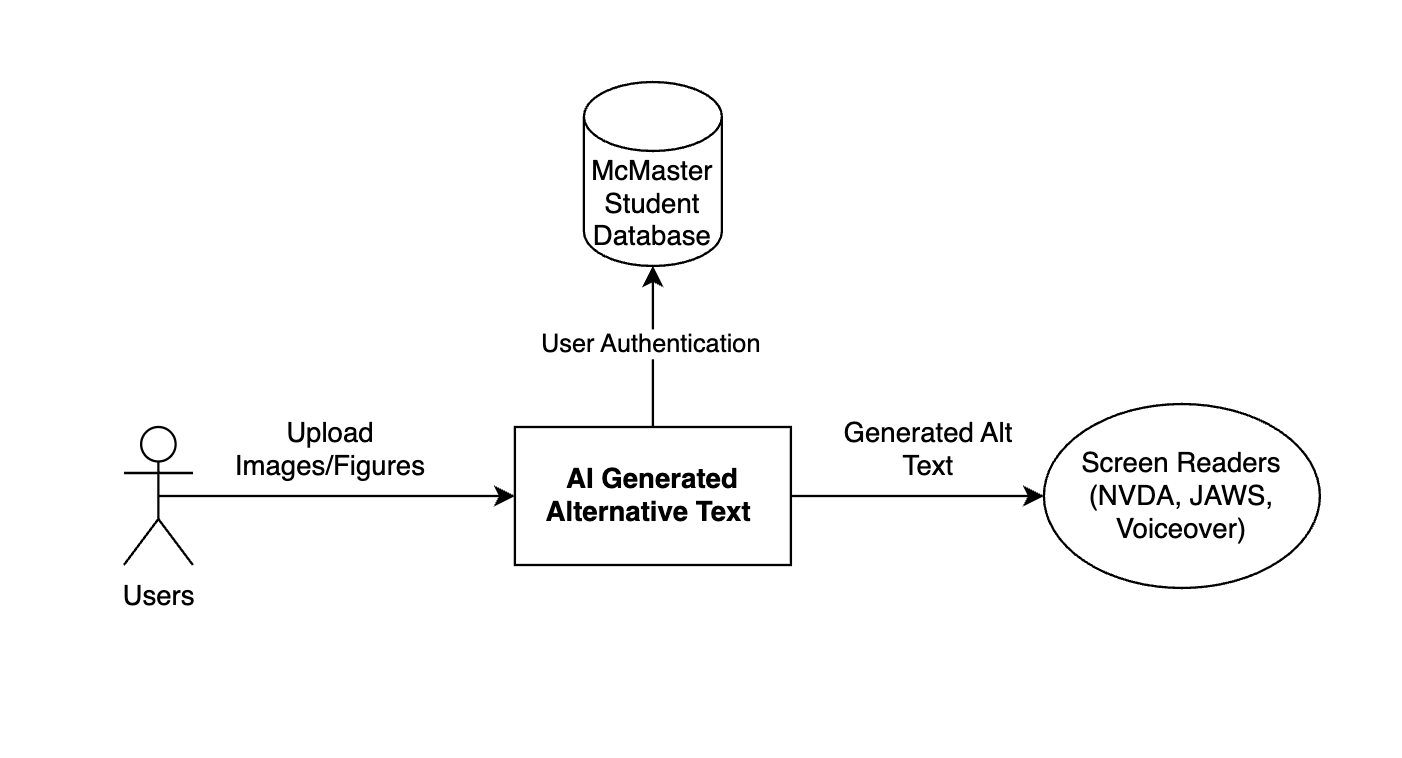
\includegraphics[width=\textwidth]{images/work-context-diagram.png}
  \caption{Work Context Diagram}
  \label{fig:work-context}
\end{figure}
\FloatBarrier   % prevents later floats from jumping before this point

\subsection{Work Partitioning}
\autoref{tab:work-partition} shows the work partitioning for
completing the project. It includes major events,
their inputs and outputs, and the summary of the event.

\begin{table}[H]
  \centering
  \caption{Work Partition for the System}
  \label{tab:work-partition}
  \begin{tabular}{ |p{3cm}|p{3cm}|p{3cm}|p{4cm}| }
    \hline
    \textbf{Event Name} & \textbf{Input} & \textbf{Output} & \textbf{Summary} \\
    \hline
    Login & Username, Password &  & User logs in using their McMaster account \\
    \hline
    Upload \mbox{Images/Figures} & PNG/JPEG files & Uploaded File
    Reference & User uploads their files to generate alternative text \\
    \hline
    \mbox{OCR Text} \mbox{Extraction} & Uploaded
    \mbox{Images/Figures} & Detected Text & System reads the text
    embedded in the uploaded files \\
    \hline
    Generate \mbox{Alternative Text} & Uploaded
    \mbox{Images/Figures}, Extracted OCR, Model Parameters &
    Generated Alt Text, Quality Metric from Machine Learning (ML)
    Model & System analyzes the image and extracted OCR data to
    generate accurate alternative text \\
    \hline
    View History & \mbox{User Login,} Stored Uploads and Generated
    Alt Text & List of Previously Generated Alt Text & The system
    retrieves and displays a user’s history of uploaded images along
    with their associated generated alt text \\
    \hline
  \end{tabular}
\end{table}

\subsection{Specifying a Business Use Case (BUC)}
The project has one primary business use case, which aims to achieve
the goal of providing users with visual and cognitive impairments an efficient
and accessible way to generate accurate alternative text for academic
images and figures.\\[1ex]
\textbf{Preconditions:}
\begin{itemize}
  \item The user has access to the web tool
  \item The user has files containing diagrams or images requiring
    alternative text
\end{itemize}
\textbf{Scenario:}
\begin{enumerate}
  \item The user logs into the system using their McMaster student credentials
  \item The user uploads one or more files (PNG, JPEG) containing diagrams
  \item The AI model analyzes the uploaded file(s), performs OCR to
    extract any visible text, and generates
    alternative text describing each image/figure accurately
  \item Screen readers use the generated alternative text to read
    aloud and convey the uploaded image
  \item The generated alternative text can be edited, copied, or
    dowloaded as a \texttt{.txt} file by the user if needed
  \item The user can view previously uploaded files and generated
    alternative text for future reference
\end{enumerate}
\textbf{Postcondition:}
\begin{itemize}
  \item The user obtains accurate and accessible alternative text
    that complies with AODA and WCAG 2.1 standards.
\end{itemize}

\section{Business Data Model and Data Dictionary}
\subsection{Business Data Model}
\lips
\subsection{Data Dictionary}
\lips

\section{The Scope of the Product}
\subsection{Product Boundary}
\autoref{fig:product-boundary} below shows the components within the system and how they connect. The components that this project will aim on building include a user interface, an alternative text generation ML model, a session history manager. Furthermore, these components will utilize or communicate with a screen reader software, McMaster Authentication system and external AI/ML Frameworks. 
\label{tab:product-boundary} 
\begin{figure}[H]
    \centering
    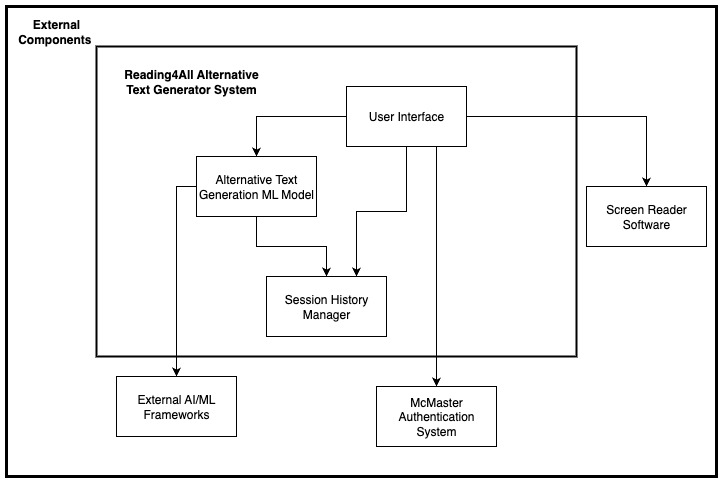
\includegraphics[width=1.0\textwidth]{images/Product_Boundary_Diagram.jpg}
    \caption{Product Boundary Diagram}
    \label{fig:product-boundary}
\end{figure}

\subsection{Product Use Case Table}
\autoref{tab:product-use} summarizes the main product use cases
for the systems. For each use case it describes the actors involved,
inputs and outputs to the system and the related requirements.
\begin{table}[H]
  \centering
  \caption{Product Use Case Table}
  \label{tab:product-use}
  \begin{tabular}{|p{1.3cm}|p{2.5cm}|p{3cm}|p{4cm}|p{2.6cm}|}
    \hline
    \textbf{PUC\#} & \textbf{PUC Name} & \textbf{Actor(s)} &
    \textbf{Input \& Output(s)} & \textbf{Requirement} \\
    \hline
    PUC 1 & Login Using McMaster Credentials &  McMaster Student and
    Faculty , McMaster Authentication System & User Credentials
    (input), Authentication Results (output) & FR 6, SR-AR 1\\
    \hline
    PUC 2 & Upload Image & McMaster Student and Faculty & JPEG or PNG
    (input), Image upload status (output) & FR 1, UHR-EUR 3 \\
    \hline
    PUC 3 & Generate Alternative Text &  McMaster Student and
    Faculty, Alternative Text Generation Model & Uploaded image
    (input), Generated alternative text  & FR 2, FR 3\\
    \hline
    PUC 4 & Copy or Download Text & McMaster Student and Faculty &
    User decision to copy or download (input), text copied to
    clipboard or downloaded & UHR-PIR 1\\
    \hline
    PUC 5 & View History of Inputted Images and their Alternative
    Text & McMaster Student and Faculty & User request to view
    history (input), Display of previously inputted images and their
    generated text within a session & FR 5\\
    \hline
  \end{tabular}
\end{table}

\subsection{Individual Product Use Cases (PUC's)}
\textbf{PUC 1: Login Using McMaster Credentials }
\begin{quote}
  \textbf{Trigger:} User selects "Login" and is directed to McMaster
  sign in page.\\
  \textbf{Preconditions:}
  \begin{itemize}
    \item The user is registered person in McMaster system and has
      valid credentials.
  \end{itemize}
  \textbf{Actors:} McMaster Student or Faculty, McMaster
  Authentication System.\\
  \textbf{Outcome:} McMaster validates user's credentials are
  validated and they are given access to system.\\
  \textbf{Input:} McMaster System username and password. \\
  \textbf{Output:} User enters system or an error message is displayed.
\end{quote}
\textbf{PUC 2: Upload Image }
\begin{quote}
\textbf{Trigger:} User selects "Upload Image" and chooses a file.\\
\textbf{Preconditions:}
\begin{itemize}
  \item User successfully logged into the system.
\end{itemize}
\textbf{Actors:} McMaster Student or Faculty \\
\textbf{Outcome:} The selected image is uploaded and stored for later text generation.\\
\textbf{Input:} Image file (JPEG or PNG) \\
\textbf{Output:} A confirmation message is displayed if the image was successfully uploaded, or an error message otherwise is displayed.
\end{quote}
\textbf{PUC 3: Generate Alternative Text}
\begin{quote}
  \textbf{Trigger:} User selects \textit{Generate Alternative Text}
  for an uploaded image.\\
  \textbf{Preconditions:}
  \begin{itemize}
    \item A valid image has been successfully uploaded to the system.
  \end{itemize}
  \textbf{Actors:} McMaster Student or Faculty.\\
  \textbf{Outcome:} The system generates a descriptive alternative
  text for the uploaded image.\\
  \textbf{Input:} User selection to generate alternative text\\
  \textbf{Output:} Generated alternative text is displayed to the user.
\end{quote}
\textbf{PUC 4: Edit Generated Alternative Text}
\begin{quote}
\textbf{Trigger:} User decides to modify the generated alternative text before copying or downloading it.\\
\textbf{Preconditions:}
\begin{itemize}
  \item System has successfully generated alternative text for an uploaded image.
\end{itemize}
\textbf{Actors:} McMaster Student or Faculty, System User Interface \\
\textbf{Outcome:} The user edits and saves the updated alternative text. \\
\textbf{Input:} User edits to the generated alternative text.\\
\textbf{Output:} The edited alternative text is displayed to the user and stored within the session, to be copied or downloaded later.
\end{quote}
\textbf{PUC 5: Copy or Download Generated Alternative Text }
\begin{quote}
\textbf{Trigger:} User selects copy or download .txt after generating alternative text.\\
\textbf{Preconditions:}
\begin{itemize}
  \item System has successfully generated alternative text for an uploaded image.
  \item User is satisfied with generated alternative text and has made any desired changes. 
\end{itemize}
\textbf{Actors:} McMaster Student or Faculty. \\
\textbf{Outcome:} The user receives the alternative text through their preferred method. \\
\textbf{Input:} User decision to copy or download.\\
\textbf{Output:} Text is copied or downloaded as .txt file on the users device.
\end{quote}
\textbf{PUC 6: View History of Uploaded Images and Generated Alternative Text}
\begin{quote}
  \textbf{Trigger:} User selects the view history option.\\
  \textbf{Preconditions:}
  \begin{itemize}
    \item User is logged in with an active session.
    \item User has previously uploaded at least one image and
      generated text within the session.
  \end{itemize}
  \textbf{Actors:} McMaster Student or Faculty.\\
  \textbf{Outcome:} The user views a list of their images and the
  corresponding generated alternative text within the current session. \\
  \textbf{Input:} User request to view session history.\\
  \textbf{Output:} Display of uploaded images and their corresponding
  generated alternative text.\\
\end{quote}

\section{Functional Requirements}
\subsection{Functional Requirements}
\begin{enumerate}[label=FR \arabic*., wide=0pt, leftmargin=*]
  \item \emph{The system must accept technical diagrams in the format
    of JPEG and PNG.}\\[2mm]
    {\bf Rationale:} The system must process JPEG/PNG images in order
    to output alternative text. \\
    {\bf Fit Criterion:} The system successfully takes as accepts
    JPEG/PNG images and provides feedback to users when an invalid
    file type is inputted.  \\
    {\bf Priority:} High
  \item \emph{The system shall generate alternative text of uploaded
    images.}\\[2mm]
    {\bf Rationale:} The main purpose of the system is to make
    scientific diagrams more accessible by generating better
    alternative-text. \\
    {\bf Fit Criterion:} For a set of test diagrams, the alternative
    text generated must meet the pre-determined criteria.\\
    {\bf Priority:} High
  \item \emph{The system shall output alternative text in a format
    compatible with screen readers.}\\[2mm]
    {\bf Rationale:} Students with disabilities utilize screen
    readers to access digital content; therefore, the alternative
    text must be displayed in away that enables screen readers to
    read it correctly. Furthermore, if the alternative text output
    format is not compatible with screen readers, then students
    cannot benefit from the application output.\\
    {\bf Fit Criterion:} The alternative text output must be readable
    by at least three commonly used screen readers.\\
    {\bf Priority:} High
  \item \emph{The system shall allow users to edit the outputted
    alternative texts.}\\[2mm]
    {\bf Rationale:} Providing users with an option to edit the
    outputted text, enables them to adjust the output to better meet
    their needs if needed.\\
    {\bf Fit Criterion:} Users can add or delete text in any part of
    the outputted alternative text and save their changes.\\
    {\bf Priority:} High
  \item \emph{The system shall store and display all inputted images
    and their generated alternative texts within a session.}\\[2mm]
    {\bf Rationale:} Storing previously inputted images and their
    generated alternative texts, allows users to easily review or
    reuse them without re-uploading. \\
    {\bf Fit Criterion:} Users can see view all previously inputted
    images with their generated alternative texts during the same session. \\
    {\bf Priority:} Medium
  \item \emph{The system must validate users during login to confirm
    they are McMaster University students.}\\[2mm]
    {\bf Rationale:} User verification will ensure that only McMaster
    University students have access to the system, ensuring that the
    system is used by the intended users.  \\
    {\bf Fit Criterion:} Users can only gain access to the system
    features after their McMaster University credentials are
    successfully validated.  \\
    {\bf Priority:} High
\end{enumerate}

\section{Look and Feel Requirements}
\subsection{Appearance Requirements}
\begin{enumerate}[label=LFR-AR \arabic*., wide=0pt, leftmargin=*]
  \item \emph{The system must allow all text on the interface to be resized up to MAX\_ZOOM\_PERCENTAGE, without any loss of functionality or content. }\\[2mm] 
    {\bf Rationale:} Allowing text resizing will enable users with low vision to more easily utilize the system. This also ensures the system meets WCAG 2.1 Success Criterion 1.4.4 Resize Text.
    User verification will ensure that only McMaster University students have access to the system, ensuring that the system is used by the intended users.  \\
    {\bf Fit Criterion:} All text, excluding any captions and images of text can be enlarged to MAX\_ZOOM\_PERCENTAGE on a standard browser zoom (ex. Google Chrome) without any overlapping, hidden content, or broken features.  \\
    {\bf Priority:} High
  \item \emph{The system must not use color as the only method to
    provide information, indicate actions or prompt user input.}\\[2mm]
    {\bf Rationale:} Users with color vision deficiencies or other
    visual impairments may not detect color differences accurately.
    This also ensures the system meets WCAG 2.1 Success Criterion
    1.4.1 Use of Color.\\
    {\bf Fit Criterion:} Any use of color communicates information to
    the user or requests information from he user must be appear with text.  \\
    {\bf Priority:} High
  \item \emph{The system must ensure sufficient contrasts of text and images of text.}\\[2mm] 
    {\bf Rationale:} Sufficient color contrast is important as it enables users with low vision or color vision deficiencies to easily read any system text. This also ensures the system meets WCAG Success Criterion 1.4.3 Contrast (Minimum)\\
    {\bf Fit Criterion:}  All text and images of text in the system interfaces has a contrast ratio of at least MIN\_CONTRAST\_RATIO.  \\
    {\bf Priority:} High
  \item \emph{The system must provide alternative text for all
    non-text content.}\\[2mm]
    {\bf Rationale:} Users with visual impairment often use screen
    readers to navigate through software systems; therefore, it is
    essential that all images have sufficient alternative text, so
    that the purpose of the images can understood. This also ensures
    the system meets WCAG Success Criterion 1.1.1 Non-text Content  .\\
    {\bf Fit Criterion:} All decorative images and non-text elements
    have alternative text that communicate their meaning. \\
    {\bf Priority:} High
\end{enumerate}

\subsection{Style Requirements}
\begin{enumerate}[label=LFR-SR \arabic*., wide=0pt, leftmargin=*]
  \item \emph{The system interface must follow a simple and modern
    design style.}\\[2mm]
    {\bf Rationale:} A simple interface will improve the systems
    usability as it better highlights the system's features, while
    also ensuring the system is visually appealing.\\
    {\bf Fit Criterion:} The system uses a clean layout with a
    maximum of three colors, consistent font styles and sizes, as
    well as only has key design elements that support usability. \\
    {\bf Priority:} High
\item \emph{The system interface must use McMaster University branding while maintaining accessibility standards and a modern style.}\\[2mm] 
    {\bf Rationale:} As the system is targeted towards McMaster University students, using the schools branding will build trust with users and ensure the system aligns with McMaster's identify. However, using McMaster branding must not interfere with usability and accessibility criteria..\\
    {\bf Fit Criterion:} The system interface includes McMaster University' official logo and meets the WCAG 2.1 contrast and non-text content success criteria. \\
    {\bf Priority:} High
\item \emph{The system interface must follow Don Norman's principles of designing an interface.}\\[2mm] 
    {\bf Rationale:} Applying Norman's principles, including visibility, feedback, constraints, mapping, consistency, and affordance, will make the system intuitive and user-friendly.\\
    {\bf Fit Criterion:} Evaluation against Norman's principles reveals no issues with any interface elements.\\
    {\bf Priority:} High
\end{enumerate}

\section{Usability and Humanity Requirements}
\subsection{Ease of Use Requirements}
\begin{enumerate}[label=UHR-EUR \arabic*., wide=0pt, leftmargin=*]
\item \emph{The system interface must allow users to efficiently use the system features.}\\[2mm] 
    {\bf Rationale:} It is important the users can quickly access and use the system features, as they may be generating multiple alternative text outputs in a single session. \\
    {\bf Fit Criterion:} Users can upload images to the system and generate alternative text in MAX\_UPLOAD\_STEPS or fewer. \\
    {\bf Priority:} High
\item \emph{The system interface must be easy for users to remember how to use after not using it for some time.}\\[2mm] 
    {\bf Rationale:} Users should be able to quickly recall how to use the system without needing to relearn the features. An intuitive design will make it easier for returning users to find and use key features.  \\
    {\bf Fit Criterion:} Users who have not used the system in a month, can successfully login, upload an image and generate alternative text within MAX\_MINUTES, without needing any assistance. \\
    {\bf Priority:} Medium
\item \emph{The system interface must provide users with clear and immediate feedback for all actions.}\\[2mm] 
    {\bf Rationale:} Providing the users with feedback ensures they understand the outcome of their actions and whether they are using the system correctly. This reduces the Gulf of Evaluation as it makes users more confident while using the system. \\
    {\bf Fit Criterion:} The system provides textual feedback within 1 second after a user interaction, such as uploading an image.  \\
    {\bf Priority:} High 
\item \emph{The system interface must provide clear instructions, prevent common errors and allow users to easily correct them.}\\[2mm] 
    {\bf Rationale:} Providing easy to follow instructions will help ensure that users can easily use the system features and prevent errors. Additionally, if a user makes a mistake, they should easily be able to revert it.  \\
    {\bf Fit Criterion:} In user testing, at least USERS\_SUCCESS\_PERCENT of users can complete tasks without errors. When a user error occurs, the system explains the issue and how to recover within MAX\_ERROR\_RECOVER.\\
    {\bf Priority:} High 
\end{enumerate}

\subsection{Personalization and Internationalization Requirements}
\begin{enumerate}[label=UHR-PIR \arabic*., wide=0pt, leftmargin=*]
\item \emph{The system interface must allow users to choose how generated alternative text is stored or copied.}\\[2mm] 
    {\bf Rationale:} Providing users with the option to either copy generated text or download it as file, helps tailor the output to the users specific needs.  \\
    {\bf Fit Criterion:} After generating the alternative text users can choose to copy or download as .txt" from the interface and system successfully completes the chosen option.\\
    {\bf Priority:} High
\end{enumerate}

\subsection{Learning Requirements}
\begin{enumerate}[label=UHR-LR \arabic*., wide=0pt, leftmargin=*]
\item \emph{The system must be easy for low-vision users to learn and operate with screen readers.}\\[2mm] 
    {\bf Rationale:} The system should be intuitive for users with low vision to use without prior training. Additionally, the system being highly compatible with screen readers, allows users to more easily navigate and use the system.  \\
    {\bf Fit Criterion:} In user testing, at least LEARNING\_PERCENT of first time users with low vision using a screen reader can upload an image and generate alternative text within MAX\_LEARNING\_MINUTES without assistance. \\
    {\bf Priority:} High
\end{enumerate}

\subsection{Understandability and Politeness Requirements}
\begin{enumerate}[label=UHR-LR \arabic*., wide=0pt, leftmargin=*]
  \item \emph{The system must only display essential information and
    hide all technical details.}\\[2mm]
    {\bf Rationale:} The system should only communicate the
    information needed to use the system. Displaying any technical
    details may cause the user to be confused and make the system
    less usable.   \\
    {\bf Fit Criterion:} In user testing, users do not encounter any
    technical terms, code outputs or information that is not relevant
    to them.  \\
    {\bf Priority:} High
\end{enumerate}

\subsection{Accessibility Requirements}
\begin{enumerate}[label=UHR-AR \arabic*., wide=0pt, leftmargin=*]
  \item \emph{The system must meet the WCAG 2.1 Level AA
    accessibility standards.}\\[2mm]
    {\bf Rationale:} The Accessibility for Ontarians with
    Disabilities Act (AODA) requires organizations to meet WCAG 2.0
    Level AA for web tools. Therefore, meeting WCAG 2.1 Level AA
    ensures the system meets AODA standards and is accessible for
    users with disabilities.  \\
    {\bf Fit Criterion:} The system will be evaluated using an
    accessibility testing tool such as Pope Tech and Wave Web Aim to
    ensure WCAG 2.1 criteria is met.\\
    {\bf Priority:} High
  \item \emph{The system must accept keyboard input for navigation.}\\[2mm]
    {\bf Rationale:} Many users, including those with disabilities,
    use keyboard inputs to navigate through applications, the system
    must support this as a way to navigate.\\
    {\bf Fit Criterion:} Users can navigate to all the main functions
    and areas of the system using their keyboard. \\
    {\bf Priority:} High
\end{enumerate}

\section{Performance Requirements}

\subsection{Speed and Latency Requirements}
\begin{itemize}
  \item[\textbf{PR-SL 1.}] \textit{The tool shall generate alt-text
    for uploaded images within a reasonable time frame.}\\
    \textbf{Rationale:} Ensures users, including those using
    assistive technologies, do not experience delays that hinder
    accessibility.\\
    \textbf{Fit Criterion:} The system shall return generated
    alt-text within \textbf{3 seconds} for images $\leq$2 MB and
    within \textbf{8 seconds} for images $\leq$10 MB under normal
    load conditions.\\
    \textbf{Priority:} High

  \item[\textbf{PR-SL 2.}] \textit{The web interface shall load and
    render accessibility components efficiently.}\\
    \textbf{Rationale:} Improves user experience and responsiveness
    for screen-reader users and keyboard navigation.\\
    \textbf{Fit Criterion:} All interactive elements shall respond
    within \textbf{300 ms} of user input under typical conditions.\\
    \textbf{Priority:} Medium
\end{itemize}

\subsection{Safety-Critical Requirements}
\begin{itemize}
  \item[\textbf{PR-SCR 1.}] \textit{The tool shall ensure that no
      personally identifiable data from uploaded images is stored or
    shared without consent.}\\
    \textbf{Rationale:} Protects user privacy and adheres to ethical
    AI standards.\\
    \textbf{Fit Criterion:} Uploaded images are deleted from
    temporary storage within \textbf{60 seconds} of processing unless
    explicitly saved by the user.\\
    \textbf{Priority:} High

  \item[\textbf{PR-SCR 2.}] \textit{The tool shall not produce
    alt-text containing offensive, biased, or harmful language.}\\
    \textbf{Rationale:} Ensures ethical AI output and inclusivity.\\
    \textbf{Fit Criterion:} 0 \% of generated outputs shall contain
    content flagged by moderation filters as offensive or biased.\\
    \textbf{Priority:} High

  \item[\textbf{PR-SCR 3.}] \textit{The interface shall adhere to
      WCAG 2.1 Level A accessibility guidelines to prevent stress or
    strain on users’ eyes and ensure comfortable interaction.}\\
    \textbf{Rationale:} Provides a visually safe, inclusive
    experience for all users, including those with visual or
    cognitive impairments.\\
    \textbf{Fit Criterion:} Verified through front-end accessibility
    testing that confirms conformance with WCAG 2.1 Level A success criteria.\\
    \textbf{Priority:} High
\end{itemize}

\subsection{Precision or Accuracy Requirements}
\label{sec:PrecisionAccuracy}
\begin{itemize}
  \item[\textbf{PR-PAR 1.}] \textit{The generated alt-text shall
      adequately describe the image content with minimal omissions or
    irrelevant details.}\\
    \textbf{Rationale:} Ensures the description fulfills its
    accessibility purpose.\\
    \textbf{Fit Criterion:} At least \textbf{85 \%} of outputs rated
    “Sufficient” or better on the sufficiency scale by testers.\\
    \textbf{Priority:} High

  \item[\textbf{PR-PAR 2.}] \textit{The alt-text shall maintain
    appropriate length and readability.}\\
    \textbf{Rationale:} Prevents overly short or verbose outputs that
    reduce usability.\\
    \textbf{Fit Criterion:} $\geq$ 90 \% of outputs rated “Proper
    Length” on the user-testing scale.\\
    \textbf{Priority:} Medium

  \item[\textbf{PR-PAR 3.}] \textit{The overall accessibility and
    usability of the alt-text shall be acceptable to testers.}\\
    \textbf{Rationale:} Evaluates real-world effectiveness of
    generated descriptions.\\
    \textbf{Fit Criterion:} Median user rating $\geq$ 3 (“Mostly
    Accessible/Usable”) on the 0–3 or 0–4 scales; no outputs below 2.\\
    \textbf{Priority:} Medium
\end{itemize}

\subsection{Robustness or Fault-Tolerance Requirements}
\begin{itemize}
  \item[\textbf{PR-RFT 1.}] \textit{The system shall gracefully
    handle unsupported or corrupted image inputs.}\\
    \textbf{Rationale:} Prevents crashes and maintains system stability.\\
    \textbf{Fit Criterion:} Invalid files trigger a clear error
    message within 2 seconds without interrupting service.\\
    \textbf{Priority:} High

  \item[\textbf{PR-RFT 2.}] \textit{The backend shall recover
    automatically from isolated process failures.}\\
    \textbf{Rationale:} Ensures continued operation without developer
    intervention.\\
    \textbf{Fit Criterion:} System recovers within 5 seconds after
    fault detection.\\
    \textbf{Priority:} High
\end{itemize}

\subsection{Capacity Requirements}
\begin{itemize}
  \item[\textbf{PR-CR 1.}] \textit{The system shall support limited
    concurrent usage suitable for a proof-of-concept deployment.}\\
    \textbf{Rationale:} Demonstrates feasibility and reliability for
    initial testing without production-level scaling.\\
    \textbf{Fit Criterion:} Supports at least \textbf{5 simultaneous
    requests} with response times $\leq$ 10 seconds.\\
    \textbf{Priority:} Medium

  \item[\textbf{PR-CR 2.}] \textit{Storage shall accommodate pilot
    testing datasets.}\\
    \textbf{Rationale:} Ensures smooth prototype validation without
    capacity issues.\\
    \textbf{Fit Criterion:} The system can temporarily store metadata
    for up to \textbf{500 images per day} without data loss.\\
    \textbf{Priority:} Low
\end{itemize}

\subsection{Scalability or Extensibility Requirements}
\begin{itemize}
  \item[\textbf{PR-SER 1.}] \textit{The architecture shall allow
      integration of improved ML models or multilingual capabilities in
    future phases.}\\
    \textbf{Rationale:} Enables progressive enhancement and future
    accessibility expansion.\\
    \textbf{Fit Criterion:} New models or language modules can be
    incorporated without restructuring existing components.\\
    \textbf{Priority:} Medium
\end{itemize}

\subsection{Longevity Requirements}
\begin{itemize}
  \item[\textbf{PR-LR 1.}] \textit{The codebase shall be maintainable
      and adaptable to updates in WCAG guidelines, Python libraries,
    and ML frameworks.}\\
    \textbf{Rationale:} Ensures long-term usability and compliance
    even after the pilot phase.\\
    \textbf{Fit Criterion:} Minor updates or migrations require
    $\leq$ 2 person-days per quarter.\\
    \textbf{Priority:} Medium

  \item[\textbf{PR-LR 2.}] \textit{The prototype shall maintain
    compatibility with at least the next two Python releases.}\\
    \textbf{Rationale:} Ensures sustainability of the pilot for
    educational and testing purposes.\\
    \textbf{Fit Criterion:} Verified through annual testing on
    supported Python versions.\\
    \textbf{Priority:} Low
\end{itemize}

\section{Operatinonal and Environment Requirements}

The following operating environment requirements define the physical,
network, interfacing, and deployment contexts in which the
Reading4All system must operate reliably and efficiently.

\subsection{Expected Physical Environment}

\begin{enumerate}[label=OER-EP\arabic*., wide=0pt, leftmargin=*]
  \item \emph{The system shall be operable on standard devices
      (laptops, desktops, or servers) running common operating systems
      such as Windows, macOS, or Linux, or deployed to standard cloud
    environments (e.g., GCP, AWS, Azure).}\\[2mm]
    {\bf Rationale:} Reading4All is intended for academic and
    institutional use, where users rely on a variety of systems.
    Supporting cross-platform and cloud deployment ensures
    accessibility and flexibility.\\
    {\bf Fit Criterion:} The system runs successfully across all
    major operating systems and supported cloud environments without
    compatibility errors.\\
    {\bf Priority:} High

  \item \emph{The system shall operate effectively under normal
    indoor conditions typical of academic or office environments.}\\[2mm]
    {\bf Rationale:} As the system is designed for digital academic
    use within classrooms and offices, no specialized environmental
    setup is required.\\
    {\bf Fit Criterion:} The tool performs consistently at standard
    indoor temperatures (10°C–35°C) and lighting levels.\\
    {\bf Priority:} Low
\end{enumerate}

\subsection{Wider Environment Requirements}

\begin{enumerate}[label=OER-WE\arabic*., wide=0pt, leftmargin=*]
  \item \emph{The system shall comply with accessibility and data
      privacy regulations, including AODA, WCAG 2.1 Level AA, and
    relevant institutional privacy policies such as FIPPA.}\\[2mm]
    {\bf Rationale:} Compliance ensures digital inclusion and privacy
    protection while aligning with university and governmental
    accessibility mandates.\\
    {\bf Fit Criterion:} Independent evaluation verifies AODA and
    WCAG 2.1 Level AA compliance, and no accessibility blockers are
    found during testing.\\
    {\bf Priority:} High

  \item \emph{The system shall operate effectively within standard
    academic network environments with stable internet connectivity.}\\[2mm]
    {\bf Rationale:} Reading4All depends on cloud-based inference
    models for text generation, which require reliable network access.\\
    {\bf Fit Criterion:} The system maintains consistent API
    communication over typical university Wi-Fi or Ethernet with
    upload speeds of at least 10 Mbps.\\
    {\bf Priority:} Medium
\end{enumerate}

\subsection{Requirements for Interfacing with Adjacent Systems}

\begin{enumerate}[label=OER-IAS\arabic*., wide=0pt, leftmargin=*]
  \item \emph{The system shall integrate with learning management
      systems (LMS) such as Avenue to Learn (D2L Brightspace) for image
    uploads and alt-text retrieval.}\\[2mm]
    {\bf Rationale:} Direct LMS integration streamlines accessibility
    workflows for instructors and students.\\
    {\bf Fit Criterion:} Reading4All successfully connects to at
    least one LMS via secure API endpoints approved by the institution.\\
    {\bf Priority:} High

  \item \emph{The system shall support interoperability with
      assistive technologies such as screen readers (e.g., NVDA, JAWS,
    and VoiceOver).}\\[2mm]
    {\bf Rationale:} Screen-reader compatibility ensures generated
    text can be read aloud for visually impaired users.\\
    {\bf Fit Criterion:} Descriptions produced by Reading4All are
    correctly parsed and read by major screen readers without
    formatting issues.\\
    {\bf Priority:} High

  \item \emph{The system shall support importing diagrams in common
    formats including JPG, JPEG, and PNG.}\\[2mm]
    {\bf Rationale:} Supporting a range of standard formats allows
    instructors to use materials from multiple academic sources.\\
    {\bf Fit Criterion:} The system processes at least one valid
    sample of each format and produces accurate alternative text.\\
    {\bf Priority:} Medium

  \item \emph{The system shall optionally interface with automated
    accessibility validation tools (e.g., WAVE or Axe).}\\[2mm]
    {\bf Rationale:} Integration with automated validators aids
    instructors in verifying alt-text accessibility compliance.\\
    {\bf Fit Criterion:} Validation reports are successfully
    generated and accessible through the user interface.\\
    {\bf Priority:} Low
\end{enumerate}

\subsection{Productization Requirements}

\begin{enumerate}[label=OER-PR\arabic*., wide=0pt, leftmargin=*]
  \item \emph{The system shall be deployable as both a web
    application and an API service for institutional integration.}\\[2mm]
    {\bf Rationale:} Dual deployment ensures accessibility for
    individual users and organizations integrating accessibility workflows.\\
    {\bf Fit Criterion:} A hosted web app and functional REST API are
    accessible and validated through institutional testing.\\
    {\bf Priority:} High

  \item \emph{The system shall securely store configuration and model
    parameters in a version-controlled and scalable environment.}\\[2mm]
    {\bf Rationale:} Proper configuration management ensures
    reproducibility and secure model versioning.\\
    {\bf Fit Criterion:} Configuration files are encrypted, tracked
    via version control, and retrievable for rollback or update.\\
    {\bf Priority:} Medium
\end{enumerate}

\subsection{Release Requirements}

\begin{enumerate}[label=OER-RL\arabic*., wide=0pt, leftmargin=*]
  \item \emph{All major functionalities (image analysis, text
      generation, and accessibility validation) must be implemented,
    tested, and verified prior to release.}\\[2mm]
    {\bf Rationale:} Ensures reliable, inclusive functionality before
    public or institutional rollout.\\
    {\bf Fit Criterion:} Verification and validation (V\&V)
    documentation confirms that each functional requirement is
    successfully tested.\\
    {\bf Priority:} High

  \item \emph{The system must be ready for release by March 18, 2026,
      aligned with the McMaster University SFWRENG 4G06 Capstone final
    demonstration schedule.}\\[2mm]
    {\bf Rationale:} Aligns release timing with Capstone evaluation
    and stakeholder presentation.\\
    {\bf Fit Criterion:} The final deliverable is fully functional,
    accessible, and deployed for the 2026 demonstration.\\
    {\bf Priority:} Medium
\end{enumerate}

\section{Maintainability and Support Requirements}

These requirements ensure the Reading4All system remains
maintainable, well-supported, and adaptable to future accessibility
standards and technical advancements.

\subsection{Maintenance Requirements}

\begin{enumerate}[label=MS-MNT\arabic*., wide=0pt, leftmargin=*]
  \item \emph{The system shall be designed with modular components to
      allow independent updates to subsystems such as the front-end
      interface, image-analysis model, language-generation model, or
    accessibility validation module.}\\[2mm]
    {\bf Rationale:} Modularity minimizes maintenance effort and
    prevents regressions when individual components are updated.\\
    {\bf Fit Criterion:} Modules are separately deployable and
    testable with independent configuration files.\\
    {\bf Priority:} High

  \item \emph{All source code shall include inline documentation and
      external developer documentation stored in the project’s GitHub
    Wiki or README.}\\[2mm]
    {\bf Rationale:} Comprehensive documentation ensures
    maintainability and smooth developer onboarding.\\
    {\bf Fit Criterion:} Each function and class includes descriptive
    docstrings, and setup steps are verified by a peer review checklist.\\
    {\bf Priority:} Medium

  \item \emph{The system shall implement a CI/CD pipeline with
    automated regression and accessibility tests.}\\[2mm]
    {\bf Rationale:} Continuous testing reduces maintenance time and
    ensures stability after updates.\\
    {\bf Fit Criterion:} Each code merge triggers automated unit,
    integration, and WCAG/AODA compliance tests.\\
    {\bf Priority:} High
\end{enumerate}

\subsection{Supportability Requirements}

\begin{enumerate}[label=MS-SUP\arabic*., wide=0pt, leftmargin=*]
  \item \emph{The system shall allow users to report issues or
      feedback directly through the interface without revealing
    personal identifiers.}\\[2mm]
    {\bf Rationale:} Enables user-driven improvements while
    maintaining privacy.\\
    {\bf Fit Criterion:} Feedback forms are logged securely without
    user PII and assigned unique issue IDs.\\
    {\bf Priority:} Medium

  \item \emph{The system shall log performance and error metrics for
    debugging and continuous improvement.}\\[2mm]
    {\bf Rationale:} Monitoring key metrics helps identify
    bottlenecks and optimize performance.\\
    {\bf Fit Criterion:} Logs record API calls, latency, error rates,
    and model confidence distributions.\\
    {\bf Priority:} Medium
\end{enumerate}

\subsection{Adaptability Requirements}

\begin{enumerate}[label=MS-AD\arabic*., wide=0pt, leftmargin=*]
  \item \emph{The system shall support integration of new AI models
    or components through a standardized interface schema.}\\[2mm]
    {\bf Rationale:} A consistent interface allows easy replacement
    or upgrading of AI components.\\
    {\bf Fit Criterion:} New modules adhere to the existing JSON I/O
    structure and pass automated compatibility checks.\\
    {\bf Priority:} High

  \item \emph{The system shall allow configuration updates without
    modifying source code.}\\[2mm]
    {\bf Rationale:} Enables rapid adaptation to new accessibility or
    institutional requirements.\\
    {\bf Fit Criterion:} All configurable parameters are stored in
    editable YAML or JSON files.\\
    {\bf Priority:} Medium

  \item \emph{All major updates shall be versioned and documented
    each academic term to ensure reproducibility.}\\[2mm]
    {\bf Rationale:} Academic projects require transparent
    traceability across semesters.\\
    {\bf Fit Criterion:} Version logs include change summaries,
    affected modules, and verification results.\\
    {\bf Priority:} Medium
\end{enumerate}

\section{Security Requirements}

\subsection{Access Requirements}
\begin{itemize}
  \item[\textbf{SR-AR 1.}] \textit{The system shall restrict access
      exclusively to McMaster University users through institutional
    Single Sign-On (SSO) authentication.}\\
    \textbf{Rationale:} Restricting access ensures only authorized
    users within McMaster can use the system during the pilot phase,
    reducing the risk of unauthorized use or data exposure.\\
    \textbf{Fit Criterion:} All users must log in using verified
    McMaster SSO credentials before accessing the platform.
    Unauthenticated requests are automatically rejected.\\
    \textbf{Priority:} High

  \item[\textbf{SR-AR 2.}] \textit{All actions performed by users
    shall be tied to their authenticated session.}\\
    \textbf{Rationale:} Linking actions to a user’s authenticated
    identity enables traceability and controlled access to system features.\\
    \textbf{Fit Criterion:} Each upload or alt-text generation event
    is associated with a unique McMaster user ID through SSO session tracking.\\
    \textbf{Priority:} Medium
\end{itemize}

\subsection{Integrity Requirements}
\begin{itemize}
  \item[\textbf{SR-IR 1.}] \textit{All communication between the
      frontend, backend, and machine learning services shall use
    encrypted HTTPS (TLS 1.2 or higher).}\\
    \textbf{Rationale:} Encryption prevents interception and
    tampering of sensitive data such as authentication tokens or image files.\\
    \textbf{Fit Criterion:} All HTTP requests must be redirected to
    HTTPS; unencrypted requests are rejected by the web server.\\
    \textbf{Priority:} High

  \item[\textbf{SR-IR 2.}] \textit{Uploaded images shall remain
    unmodified during processing and analysis.}\\
    \textbf{Rationale:} Preserving file integrity ensures consistent
    and accurate generation of alt-text.\\
    \textbf{Fit Criterion:} File hash comparison verifies that image
    files remain identical throughout the upload and analysis process.\\
    \textbf{Priority:} High
\end{itemize}

\subsection{Privacy Requirements}
\begin{itemize}
  \item[\textbf{SR-PR 1.}] \textit{Uploaded images shall be deleted
    immediately after processing is complete.}\\
    \textbf{Rationale:} Protects user privacy and ensures compliance
    with institutional data governance policies.\\
    \textbf{Fit Criterion:} Uploaded files are stored temporarily in
    memory or on a secure local directory and deleted within 60
    seconds after alt-text generation.\\
    \textbf{Priority:} High

  \item[\textbf{SR-PR 2.}] \textit{Generated alt-text shall not
    contain personally identifiable information (PII) or sensitive content.}\\
    \textbf{Rationale:} Prevents disclosure of private information
    and ensures responsible AI usage.\\
    \textbf{Fit Criterion:} The model output is passed through a
    content moderation filter that rejects or flags any alt-text
    containing PII or inappropriate language.\\
    \textbf{Priority:} Medium
\end{itemize}

\subsection{Audit Requirements}
\begin{itemize}
  \item[\textbf{SR-AU 1.}] \textit{System usage logs shall record
      authentication events, uploads, and generation activities for
    accountability and debugging.}\\
    \textbf{Rationale:} Audit logs enable traceability, assist in
    debugging, and ensure ethical research practices.\\
    \textbf{Fit Criterion:} Logs record timestamps, user IDs, and
    non-sensitive metadata while excluding image or generated text content.\\
    \textbf{Priority:} Medium

  \item[\textbf{SR-AU 2.}] \textit{Access to audit logs shall be
    restricted to authorized project administrators.}\\
    \textbf{Rationale:} Limits access to potentially sensitive
    operational data and protects user confidentiality.\\
    \textbf{Fit Criterion:} Logs are stored in a restricted-access
    directory with read permissions granted only to administrators.\\
    \textbf{Priority:} Medium
\end{itemize}

\subsection{Immunity Requirements}
\begin{itemize}
  \item[\textbf{SR-IM 1.}] \textit{The system shall validate and
      sanitize all uploaded files to prevent malicious or unsupported
    file types.}\\
    \textbf{Rationale:} Protects against injection attacks, corrupted
    uploads, or execution of non-image files.\\
    \textbf{Fit Criterion:} Only files with valid image types (.png,
    .jpg, .jpeg, .svg, .webp) are accepted; unsupported or script
    files are automatically rejected.\\
    \textbf{Priority:} High

  \item[\textbf{SR-IM 2.}] \textit{The system shall block access from
    networks or domains outside McMaster University’s infrastructure.}\\
    \textbf{Rationale:} Restricting network access minimizes exposure
    to external threats during the proof-of-concept phase.\\
    \textbf{Fit Criterion:} Requests must originate from verified
    McMaster SSO tokens or IP ranges associated with university networks.\\
    \textbf{Priority:} High
\end{itemize}

\section{Cultural Requirements}
The following list conists of cultural requirements the system shall follow:
\begin{itemize}
  \item[\textbf{CR 1.}] \textit{The system shall generate alternative
      text using neutral and inclusive language appropriate for
    academic environments.}\\
    \textbf{Rationale:} Ensures that generated content is respectful
    to diverse cultural and educational backgrounds.\\
    \textbf{Fit Criterion:} Generated alt text contains no culturally
    biased, exclusionary, or inappropriate terminology.\\
    \textbf{Priority:} High

  \item[\textbf{CR 2.}] \textit{The system shall avoid using
      culturally specific references unless the visual content
    explicitly requires it.}\\
    \textbf{Rationale:} Prevents misinterpretation and maintains
    accessibility for a wide audience.\\
    \textbf{Fit Criterion:} Alt text focuses on visual description
    and context without unnecessary cultural assumptions.\\
    \textbf{Priority:} Medium

  \item[\textbf{CR 3.}] \textit{The system shall use professional and
    educationally appropriate tone in all generated content.}\\
    \textbf{Rationale:} Maintains usability across academic
    departments and contexts.\\
    \textbf{Fit Criterion:} Outputs remain formal, non-colloquial,
    and context-relevant.\\
    \textbf{Priority:} Medium
\end{itemize}

\section{Compliance Requirements}
\subsection{Legal Requirements}
\begin{itemize}
  \item[\textbf{CR-LR 1.}] \textit{The system shall comply with AODA
    standards for alternative text generation.}\\
    \textbf{Rationale:} Ensures the tool supports institutional
    accessibility requirements and legal obligations.\\
    \textbf{Fit Criterion:} All generated alt text meets WCAG 2.1
    Level AA criteria for accuracy, clarity, and relevance.\\
    \textbf{Priority:} High
\end{itemize}
\subsection{Standards Compliance Requirements}
\begin{itemize}
  \item[\textbf{CR-SCR 1.}] \textit{The system shall follow
      institutional privacy and data-handling guidelines for uploaded
    teaching materials.}\\
    \textbf{Rationale:} Prevents unauthorized distribution or
    mishandling of academic content.\\
    \textbf{Fit Criterion:} No files are stored beyond active use
    unless explicitly authorized; logs exclude proprietary content.\\
    \textbf{Priority:} High

  \item[\textbf{CR-SCR 2.}] \textit{The system shall provide verifiable
    documentation or statements of compliance upon request.}\\
    \textbf{Rationale:} Facilitates audits, approvals, and
    integration into university workflows.\\
    \textbf{Fit Criterion:} A compliance overview document or help
    section is available to stakeholders.\\
    \textbf{Priority:} Medium
\end{itemize}

\section{Open Issues}
This section outlines unresolved questions and decisions that may
impact the overall success of the system.
The following items require additional research, testing, or
discussion to ensure the project’s successful completion.
\begin{itemize}
  \item The ML/AI model architecture the team will use to generate
    alternative text will need research and testing
    to ensure optimal accuracy and correctness.
  \item The optimal length of the generated alternative text requires
    further research to determine how many characters provide an
    accurate description without causing confusion or distracting
    from the main idea of the diagram.
\end{itemize}

\section{Off-the-Shelf Solutions}

This section identifies existing tools, reusable components, and
research products that can support or inspire the development of
Reading4All. These solutions address various aspects of the system’s
vision analysis, language generation, and accessibility workflows.

\subsection{Ready-Made Products}

\begin{itemize}
  \item \textbf{Google Cloud Vision API:} A commercial computer
    vision service capable of detecting objects, text, and structural
    elements within images. It can assist in preliminary diagram
    segmentation or optical character recognition for Reading4All’s
    visual analysis component.

  \item \textbf{Microsoft Azure Cognitive Services:} Offers image
    captioning and scene-description APIs that generate textual
    summaries of visual content. These can serve as a performance
    benchmark for Reading4All’s AI-generated academic alt text.

  \item \textbf{OpenAI GPT-4V (Vision):} A multimodal AI model
    capable of interpreting images and generating context-aware
    captions. It can be evaluated for use in academic diagrams and as
    a reference for Reading4All’s natural-language generation pipeline.
\end{itemize}

\subsection{Reusable Components}

\begin{itemize}
  \item \textbf{Hugging Face Transformers:} An open-source library
    offering pretrained multimodal models (e.g., BLIP-2, CLIP, and
    ViT-GPT2). These can be fine-tuned to identify structural and
    semantic relationships within STEM diagrams.

  \item \textbf{Albumentations:} A Python library for data
    augmentation, enhancing dataset diversity for diagram recognition
    tasks. It can be reused in Reading4All’s preprocessing pipeline
    to improve robustness.

  \item \textbf{Pandas + Matplotlib AltText Plugin:} An open-source
    extension that generates descriptive alt text for statistical
    plots. Its modular logic can guide Reading4All’s diagram-specific
    description component.
\end{itemize}

\subsection{Products That Can Be Copied}

\begin{itemize}
  \item \textbf{Chart2Text:} A benchmark system that automatically
    converts data visualizations such as bar charts and line graphs
    into natural-language summaries. Its approach to aligning visual
    features with linguistic structures provides a strong foundation
    for Reading4All’s diagram-description workflow.

  \item \textbf{SciA11y:} A research initiative by the Allen
    Institute for AI that generates accessible figure descriptions
    for scientific papers. Its methods for extracting captions,
    metadata, and contextual relationships between visual and textual
    elements align closely with Reading4All’s academic accessibility objectives.
\end{itemize}
\section{Tasks}

\subsection{Project Planning}

\begin{itemize}
  \item \textbf{Development Approach}
    The Reading4All team will follow an iterative agile workflow
    emphasizing continuous improvement and regular feedback from
    stakeholders. Development will progress through a series of short
    sprints that each target measurable goals, allowing flexibility
    as requirements evolve. The general process will involve:
    \begin{enumerate}
      \item Requirement analysis and refinement of functional specifications
      \item Sprint planning and backlog prioritization
      \item Incremental coding and integration
      \item Verification, validation, and unit testing
      \item Periodic reviews with the project supervisor and accessibility lead
      \item System deployment and documentation finalization
    \end{enumerate}

  \item \textbf{Key Tasks}
    \begin{itemize}
      \item Confirm system architecture and interface specifications
      \item Establish a shared GitHub repository with branching standards
      \item Configure CI/CD automation through GitHub Actions
      \item Implement the vision module for diagram segmentation and labeling
      \item Integrate the language generation component for alt-text synthesis
      \item Conduct user testing with instructors and accessibility specialists
      \item Evaluate outputs for WCAG 2.1 compliance and descriptive accuracy
    \end{itemize}

  \item \textbf{Resource Estimates}
    The project involves a five-member team responsible for design,
    development, testing, and reporting. Shared tools will include:
    \begin{itemize}
      \item Cloud computing resources (GPU-based inference environment)
      \item Version control and issue tracking using GitHub Projects
      \item Datasets of academic diagrams and verified alternative texts
    \end{itemize}

  \item \textbf{Key Considerations}
    \begin{itemize}
      \item Early integration testing to avoid dependency conflicts
      \item Dataset bias evaluation to ensure inclusive model outputs
      \item Consistent communication with the faculty advisor and
        accessibility consultant
      \item Risk reduction through checkpoint testing and documentation reviews
    \end{itemize}

  \item \textbf{Documentation Process}
    \begin{itemize}
      \item Maintain all documentation collaboratively within the GitHub Wiki
      \item Use meaningful commit messages and structured pull requests
      \item Require automated testing to pass before merging any code
      \item Apply peer review and version tagging for every major deliverable
      \item Archive final reports and test results for supervisor review
    \end{itemize}
\end{itemize}

\subsection{Planning of the Development Phases}

\textbf{Deliverables and Tentative Schedule}

\begin{itemize}
  \item Problem Statement, Proof of Concept, and Development Plan —
    \textbf{Week 4 (September 24, 2025)}
  \item Software Requirements Specification (SRS) and Hazard Analysis
    — \textbf{Week 6 (October 8, 2025)}
  \item Verification and Validation Plan — \textbf{Week 8 (October 22, 2025)}
  \item Design Document (Revision 0) — \textbf{Week 10 (November 5, 2025)}
  \item Proof of Concept Demonstration — \textbf{Weeks 11–12
    (November 12–19, 2025)}
  \item Design Document (Revision 1) — \textbf{Week 16 (January 21, 2026)}
  \item Revision 0 Demonstration — \textbf{Weeks 18–19 (February 4–11, 2026)}
  \item Verification and Validation Report — \textbf{Week 22 (March 4, 2026)}
  \item Final Demonstration (Revision 1) — \textbf{Week 24 (March 18, 2026)}
  \item Capstone EXPO — \textbf{Week 26 (April 1, 2026)}
  \item Final Documentation Submission — \textbf{Week 26 (April 1, 2026)}
\end{itemize}

\textbf{Sprint and Review Cycle}
\begin{itemize}
  \item Each sprint will run for approximately two weeks, concluding
    with a progress review.
  \item Development milestones will be validated through automated
    testing and peer evaluation.
  \item Supervisor and accessibility advisor feedback will guide
    milestone adjustments and task prioritization.
\end{itemize}

By adopting this structured development plan, the team will ensure
that Reading4All evolves into a reliable and maintainable system
capable of producing accurate, accessible, and pedagogically useful
alt text for academic diagrams.

\section{Migration to the New Product}
\subsection{Requirements for Migration to the New Product}
\begin{itemize}
  \item[\textbf{MNP-RMNP 1.}] \textit{The system shall support a
      phased implementation to allow gradual adoption while minimizing
    disruptions.}\\
    \textbf{Rationale:} Reduces organizational risk and allows
    controlled testing during rollout.\\
    \textbf{Fit Criterion:} Each phase is deployed and validated
    independently before progressing to the next.\\
    \textbf{Priority:} High

  \item[\textbf{MNP-RMNP 2.}] \textit{The organization shall operate
      the new system in parallel with the old product for a defined
    transition period.}\\
    \textbf{Rationale:} Ensures continuity and confirms correct
    operation before full cutover.\\
    \textbf{Fit Criterion:} Parallel operation lasts until all
    critical functions pass acceptance testing.\\
    \textbf{Priority:} High

  \item[\textbf{MNP-RMNP 3.}] \textit{The system shall provide
    procedures and tools for manual backup during transition.}\\
    \textbf{Rationale:} Maintains operational stability during migration.\\
    \textbf{Fit Criterion:} Backup processes are documented, tested,
    and accessible to staff.\\
    \textbf{Priority:} Medium

  \item[\textbf{MNP-RMNP 4.}] \textit{The transition plan shall
    identify and schedule major components and release phases.}\\
    \textbf{Rationale:} Guides project planning and resource allocation.\\
    \textbf{Fit Criterion:} A migration timeline with milestones and
    dependencies is documented.\\
    \textbf{Priority:} Medium
\end{itemize}

\subsection{Data That Has to be Modified or Translated for the New System}
This section does not apply to this project as there is no current
system to replace, thus, no data at all.

\section{Costs}

The total cost of developing this project is primarily based on the
effort contributed by the student development team and faculty
supervisors. As the project utilizes open-source technologies (e.g.,
Python, TensorFlow, Flask, and React) and university-hosted
infrastructure, no direct monetary expenditure is incurred. The
project is scheduled to be completed within the academic term (MVP
ready by April 2026), and resource allocation is focused on efficient
time management and workload balancing rather than financial cost.

\subsection{Metrics for Estimation}

To estimate overall development cost in terms of time and effort, the
following key metrics have been considered:
\begin{itemize}
  \item Number of image input/output workflows supported by the tool.
  \item Number of core functional requirements (e.g., image upload,
    alt-text generation, user authentication, evaluation metrics).
  \item Number of non-functional requirements (e.g., accessibility
    compliance, latency, privacy, and scalability).
  \item Number of deliverables and milestones within the development timeline.
  \item Team size and individual role distribution (frontend,
    backend, model integration, documentation).
\end{itemize}

\subsection{Estimation Approach}

Each deliverable has been estimated based on the effort required to
implement, test, and document it within the given academic term.
The estimates are derived from prior experience with similar
web-based machine learning projects and adjusted for the learning and
research effort required to integrate accessibility and WCAG
compliance features.
Time allocation also accounts for model fine-tuning, front-end
accessibility testing, and usability evaluation with pilot users.

\subsection{Cost Breakdown}

\noindent\textbf{• Development Effort:} Based on a team of four
student developers and one faculty supervisor, the estimated time
allocation per team member is as follows:
\begin{itemize}
  \item Initial research, planning, and requirement analysis:
    \textbf{40 hours per team member.}
  \item Model integration and backend implementation: \textbf{120
    hours per team member.}
  \item Frontend development and accessibility compliance: \textbf{80
    hours per team member.}
  \item Testing, debugging, and refinement: \textbf{60 hours per team member.}
  \item Documentation and presentation preparation: \textbf{30 hours
    per team member.}
\end{itemize}
\noindent\textbf{Total estimated effort: 330 hours per team member.}

\noindent\textbf{• Tools and Software:}
All software components used in the project (Python, Flask, React,
TensorFlow, Machine Learning Models, and GitHub) are open-source or
free for academic use.
Therefore, there are no direct licensing or software procurement costs.

\noindent\textbf{• Testing Environment:}
Testing will be conducted using McMaster-hosted or open-source
platforms for model inference and user testing.
The team might decide to conduct user testing and award attendees 10
dollar Amazon.com gift cards as a reward for participation.
No additional hardware purchases are required beyond existing student
laptops and cloud compute credits provided for academic purposes.

\subsection{Estimated Cost}

The total development effort is estimated at approximately
\textbf{1,320 person-hours} across all team members (4 × 330 hours).
Assuming an average academic hourly equivalent of \textbf{\$20 per
hour} for estimation purposes, the notional cost of development would
be approximately \textbf{\$26,400 CAD}.

However, as this project is conducted as part of a capstone academic
course and leverages free university and open-source resources, the
\textbf{actual monetary cost is \$0 CAD}.
The effective cost of the project lies entirely in time, research,
and human effort required to meet the performance, accessibility, and
security requirements outlined in previous sections.

\section{User Documentation and Training}
\subsection{User Documentation Requirements}
\begin{enumerate}
  \item User Manual
    \begin{itemize}
      \item \textbf{Purpose}: The user manual will serve as a user
        guide and provide detailed information and instructions on
        the final product and how to use it effectively
      \item \textbf{Target Audience}: Academic students, instructors,
        and other professionals
      \item \textbf{Content}: Web tool navigation and instructions,
        usage examples, product purposes, and best practices
    \end{itemize}
\end{enumerate}
\subsection{Training Requirements}
Users of the final product will require minimal to no training as we
aim to ensure that the tool is as accessible, simple, and intuitive
as possible. For any additional guidance,
a user manual will be created along with any relevant tutorials on
how to use the features within the web tool.

\section{Waiting Room}
This section lists potential ideas and features that are out of scope
for the current project, however, may be valuable for future updates.
\begin{itemize}
  \item Support for multilingual alternative text generation (e.g.,
    French and Spanish)
  \item A browser extension that automatically generates alternative
    text on websites or learning platforms (e.g. \textit{D2L}) using our model
  \item Compatibility with mobile platforms to extend accessibility
    across users' preferred devices
\end{itemize}

\section{Ideas for Solution}
This section discusses potential ways to achieve some of the functionality discussed throughout this report, 
including image upload and processing, alternative text generation and session history. 
These ideas have been documented so they can be referenced later during development.\\
This section discusses potential ways to acheive some of the
functionality discussed throughout this report,
including image upload and processing, alternative text generation
and session history.
These ideas have been documented so they can be referenced later
during development.\\
\\
\textbf{Image Upload and Processing}
This functionality can be achieved through a front-end interface,
where users are prompted to upload an image using an upload button or
by dragging their file into the drop box. Furthermore, to minimize
errors, this will only allow JPEG and PNG image files.
Once the image has been uploaded, it will be displayed to the user
with the image file name, so users can confirm the correct file was chosen.
If the upload fails, the system will display an error message
explaining the issue. Furthermore, this can be achieved using the
HTML5 File API, which supports reading and processing file data,
specifically obtained through input or drag and drop. \\
\\
\textbf{Alternative Text Generation}
This functionality can be implemented using a vision-language model
(VLM), which combines natural language models with computer vision.
The model can learn from both images and text to solve various
problems. The model can be trained using sample scientific images,
paired with examples of descriptive alternative text, allow it to
generate accurate and high quality descriptions for new images.\\
\\
\textbf{Session History}
After the user is satisfied with the generated alternative text, the
system will store the image and its final description in the
browser's session storage as a JSON record. This allows the data to
be stored temporarily and can easily be displayed to the user when
they request their history. \\
\section*{Appendix --- Reflection}

The purpose of reflection questions is to give you a chance to assess your own
learning and that of your group as a whole, and to find ways to improve in the
future. Reflection is an important part of the learning process.  Reflection is
also an essential component of a successful software development process.  

Reflections are most interesting and useful when they're honest, even if the
stories they tell are imperfect. You will be marked based on your depth of
thought and analysis, and not based on the content of the reflections
themselves. Thus, for full marks we encourage you to answer openly and honestly
and to avoid simply writing ``what you think the evaluator wants to hear.''

Please answer the following questions.  Some questions can be answered on the
team level, but where appropriate, each team member should write their own
response:

\textbf{Group Reflection  - Reflection}
\begin{enumerate}
  \item What went well while writing this deliverable? 
  
  Throughout the process, our team maintained organization and had good communication.  It was simpler to preserve flow and prevent redundancy because we had a clear framework and consistent formatting from earlier deliverables.  We were also able to maintain our efficiency and keep the material consistent with our previous work.  In order review sections, define expectations, and make sure the deliverable satisfied all requirements, we also had meetings with our TA and our team.
  \item What pain points did you experience during this deliverable, and how did
  you resolve them?

  One difficulty was avoiding redundancy by keeping formatting constant and clearly distinguishing design components from implementation specifics. In order to guarantee accuracy and uniformity throughout all sections, we addressed this by going over the course templates and conducting team editing sessions to make sure the formatting followed a consistent style. We also helped each other out by sharing tips and tricks to improve clarity and presentation.

  \item How many of your requirements were inspired by speaking to your
  client(s) or their proxies (e.g. your peers, stakeholders, potential users)?
  
  Key design and functionality components that were influenced by internal meetings, conversations with our supervisor, pertinent compliance guidelines, and my internship's prior experience working with AI included the accessible interface, the quality of the alt text that was generated, and adherence to AODA and WCAG 2.1 standards.
  \item Which of the courses you have taken, or are currently taking, will help
  your team to be successful with your capstone project.

  The Software Requirements course from third year was extremely useful in creating this deliverable.  It created a solid foundation for organizing requirement documents, developing precise specifications, and grasping the foundations of software documentation and traceability, all of which significantly aided our work on this project.

  \item What knowledge and skills will the team collectively need to acquire to
  successfully complete this capstone project?  Examples of possible knowledge
  to acquire include domain specific knowledge from the domain of your
  application, or software engineering knowledge, mechatronics knowledge or
  computer science knowledge.  Skills may be related to technology, or writing,
  or presentation, or team management, etc.  You should look to identify at
  least one item for each team member.}\newline
  
  \item \textbf{For each of the knowledge areas and skills identified in the previous
  question, what are at least two approaches to acquiring the knowledge or
  mastering the skill?  Of the identified approaches, which will each team
  member pursue, and why did they make this choice?}\newline

\end{enumerate}


\textbf{Moly Mikhail  - Reflection}
\begin{enumerate}
  \item \textbf{What went well while writing this deliverable?} \newline
  I believe writing this deliverable many things went well. I really enjoyed getting to think about the different
  non-functional requirements. I found that have different sections of non-functional requirements encouraged me to think about different 
  aspects of the system and things we will have to keep in mind during development. For example, prior to writing 
  this deliverable, we hadn’t considered personalization and internationalization requirements; however, having to
  complete that section led us to add important functionality of allowing the user to decide which way
  to store the alternative text. 
  
\item \textbf{What pain points did you experience during this
    deliverable, and how did you resolve them?} \newline
  One pain point I experience writing this deliverable dealt with completing the product boundary. 
  Initially, I was confused on The Scope of the Product section and what was expected. 
  To resolve this, I researched the Volere Requirements Specification Template and looked into the section. 
  However, I was still confused and what was expected of the section. Finally, during our meeting with
  our TA I was able to clarify the expectations for this section and I was able to complete the section. 
 
   \item \textbf{How many of your requirements were inspired by
      speaking to your client(s) or their proxies (e.g., your peers,
    stakeholders, potential users)?} \newline
  I believe many of our non-functional requirements, specifically look and feel 
  requirements, as well as usability and humanity requirements. Through our
  conversations with our supervisor Jing, we learned a lot of the accessibility
  requirements for website applications. For example, one specific requirement 
  that was derived from our conversations was that the system cannot use color alone to convey any messages
  or information. I believe without having this conversation, this is a requirement that would not have been discovered. 
 
 \item \textbf{Which of the courses you have taken, or are currently
      taking, will help your team be successful with your capstone
    project?} \newline
  I believe many courses that I have taken, and some that I’m currently taking will 
  contribute to the success of our capstone project. I completed
  SFWRENG 4HC3 - Human Computer Interfaces, which has taught me many 
  important design principles, such as Normans Design Principles. Furthermore, 
  completing COMPSCI 4AL3 - Applications of Machine Learning, also will be a lot of help when 
  completing our capstone. This course introduced me to developing machine learning models and 
  will be directly applicable. Finally, taking COMPSCI 3RA3 - Software Requirements and Security 
  Considerations will also help our team be successful. 
  
\end{enumerate}

\textbf{Casey Francine Bulaclac - Reflection}
\begin{enumerate}
  \item \textbf{What went well while writing this deliverable?} \newline
  Having discussed the project thoroughly as a team and with our supervisor helped in writing this deliverable as the team
  was very knowledgeable about the needs for the project. 
  This deliverable went much smoother than the last due to stronger operational procedures, and better organization in how we structured and completed the SRS. 
  The team communicated well and were clear of the goals for this deliverable.
  \item \textbf{What pain points did you experience during this
  deliverable, and how did you resolve them?} \newline
  One pain point in writing the SRS was figuring out what each of the many sections entailed in the Volere's template. The template 
  is very thorough and needed many details, in which some sections seem to overlap which can be confusing. Another pain point was ensuring traceability
  between our goals in the project and the requirements. To resolve this, I made sure to ask the TA for feedback and clarification about specific sections.
  Additionally, communicating with each team member and ensuring our requirements aligned to the goals of the project was very helpful in aiding to ensure
  traceability.
\item \textbf{How many of your requirements were inspired by
      speaking to your client(s) or their proxies (e.g., your peers,
    stakeholders, potential users)?} \newline
  Many, if not most, requirements were inspired through speaking with our supervisor, who had the most knowledge and experience with our project's 
  potential users and stakeholders. In this project, it is important to understand our target users as we are designing for accessibility, so it was critical 
  in making our requirements. 
 \item \textbf{Which of the courses you have taken, or are currently
      taking, will help your team be successful with your capstone
    project?} \newline
  In this deliverable, the course that was most beneficial was Software Requirements and Security Considerations (SFWRENG 3RA3) as we learned how to create effected SRS documents.
  A course I've taken that will help thoroughly in ensuring our user interface is accessible is Human Computer Interfaces (SFWRENG 4HC3) as the course taught us principles of good design. Lastly,
  another course I took that contribute to the success of our project is Applications of Machine Learning (SFWRENG 4AL3) as this project heavily involves machine learning
  in generating alternative text. 
\end{enumerate}

\textbf{Nawaal Fatima - Reflection}
\begin{enumerate}
  \item \textbf{What went well while writing this deliverable?} \newline
    Our group divided the work efficiently, which made the writing
    process smoother. I found that once we agreed on the structure,
    it became easier to contribute my part because everyone had a
    clear understanding of what they were responsible for.
    We all came together towards the end and reviewed everyone's
    parts, ensuring coherency and consistency in our writing.
    Communication also went well, and we were able to clarify
    uncertainties quickly through discussions. Personally, I felt
    more confident writing my section because I understood how my
    contribution fit into the overall deliverable.

  \item \textbf{What pain points did you experience during this
    deliverable, and how did you resolve them?} \newline
    One challenge I experienced was making sure my writing aligned
    with the tone and level of detail the rest of the team was using.
    At first, it was hard to tell how formal or detailed certain
    sections should be. I resolved this by checking in with my teammates'
    writing and reading over their parts so that my section matched in style.
    Another minor pain point was managing time alongside other
    coursework, but planning out smaller chunks helped me stay on track.
    Furthermore, my computer glitched during an update and I had to
    rewrite all of my sections which was super frustrating and
    delayed some teammate's sections. In the future I will ensure to
    commit all drafts to a remote branch before updating my computer.

  \item \textbf{How many of your requirements were inspired by
      speaking to your client(s) or their proxies (e.g., your peers,
    stakeholders, potential users)?} \newline
    A noticeable portion of the requirements came from talking to
    Ms. Sui and from my experiences working with her over the past
    three years. Even though we don't always interact with the customers
    directly, speaking to Ms. Sui and imagining how potential users
    would interact with the system helped shape several of the
    requirements. I'd estimate that roughly half of the requirements
    were influenced by those conversations or by feedback from people
    who could represent the end users.

  \item \textbf{Which of the courses you have taken, or are currently
      taking, will help your team be successful with your capstone
    project?} \newline
    Several courses connect directly to this project. Software
    engineering and requirements-focused courses helped with
    understanding how to draft clear specifications and think about
    users' needs. Any design or project-based courses gave me
    experience working in teams and coordinating deliverables.
    Courses that covered testing, human-computer interfaces,
    documentation, and development
    processes also helped ensure we follow good practices
    throughout the capstone.
\end{enumerate}

\newpage
\section*{References}

\begin{hangparas}{2em}{1}
  Microsoft, ``Azure AI Vision---Image Analysis,'' Microsoft Docs/Learn.
  Accessed: Oct.~9,~2025. [Online]. Available:
  \url{https://learn.microsoft.com/en-us/azure/ai-services/computer-vision/overview-image-analysis?tabs=4-0}
  \\
  \par
  AltText.ai, ``AltText.ai---Automatic Image Alt Text Generation,'' AltText.ai.
  Accessed: Oct.~9,~2025. [Online]. Available: \url{https://alttext.ai/}
  \\
  \par
  accessiBe, ``Building a more accessible web together'', accessiBe.
  Accessed: Oct.~9,~2025. [Online]. Available:
  \url{https://www.accessibe.com/about}
\end{hangparas}

\end{document}
